\documentclass[11pt, a4paper]{memoir}

%% LaTeX Font encoding -- DO NOT CHANGE
\usepackage[OT1]{fontenc}
\usepackage[english]{babel}
\usepackage[utf8]{inputenc}
\usepackage[sc]{mathpazo}
\usepackage{amsmath,amssymb,amsfonts,mathrsfs}
\usepackage[amsmath,thmmarks]{ntheorem}
\usepackage{graphicx}

% Other packages
\usepackage{caption}
\usepackage{subcaption}
\usepackage{booktabs}
\usepackage{pdfpages}
\usepackage{numprint}
\newcommand{\num}[1]{\numprint{#1}}

\usepackage{lipsum}


\usepackage[colorinlistoftodos]{todonotes}

\usepackage{datetime}
\newdateformat{mydate}{%
  \monthname[\THEMONTH] \THEDAY, \THEYEAR}

% Load hyperref last
\usepackage{hyperref}

\usepackage[capitalise, nameinlink]{cleveref}
\hypersetup{
   colorlinks=true,
    linkcolor=blue,
    citecolor=blue,
    filecolor=blue,
    urlcolor=blue,
    linktoc=all, 
    }
    
\Crefname{equation}{Equation}{Equations}
\Crefname{figure}{Figure}{Figures}
\Crefname{tabular}{Table}{Tabels}



%% Our layout configuration.  DO NOT CHANGE.
%% Memoir layout setup

% NOTE: You are strongly advised not to change any of them unless you
% know what you are doing.  These settings strongly interact in the
% final look of the document.

% Dependencies
% Turn extra space before chapter headings off.
\setlength{\beforechapskip}{0pt}

\nonzeroparskip
\parindent=0pt
\defaultlists

% Chapter style redefinition
\makeatletter

\if@twoside
  \pagestyle{Ruled}
  \copypagestyle{chapter}{Ruled}
\else
  \pagestyle{ruled}
  \copypagestyle{chapter}{ruled}
\fi
\makeoddhead{chapter}{}{}{}
\makeevenhead{chapter}{}{}{}
\makeheadrule{chapter}{\textwidth}{0pt}
\copypagestyle{abstract}{empty}

\makechapterstyle{bianchimod}{%
  \chapterstyle{default}
  \renewcommand*{\chapnamefont}{\normalfont\Large\sffamily}
  \renewcommand*{\chapnumfont}{\normalfont\Large\sffamily}
  \renewcommand*{\printchaptername}{%
    \chapnamefont\centering\@chapapp}
  \renewcommand*{\printchapternum}{\chapnumfont {\thechapter}}
  \renewcommand*{\chaptitlefont}{\normalfont\huge\sffamily}
  \renewcommand*{\printchaptertitle}[1]{%
    \hrule\vskip\onelineskip \centering \chaptitlefont\textbf{\vphantom{gyM}##1}\par}
  \renewcommand*{\afterchaptertitle}{\vskip\onelineskip \hrule\vskip
    \afterchapskip}
  \renewcommand*{\printchapternonum}{%
    \vphantom{\chapnumfont {9}}\afterchapternum}}

% Use the newly defined style
\chapterstyle{bianchimod}

\setsecheadstyle{\Large\bfseries\sffamily}
\setsubsecheadstyle{\large\bfseries\sffamily}
\setsubsubsecheadstyle{\bfseries\sffamily}
\setparaheadstyle{\normalsize\bfseries\sffamily}
\setsubparaheadstyle{\normalsize\itshape\sffamily}
\setsubparaindent{0pt}

% Set captions to a more separated style for clearness
\captionnamefont{\sffamily\bfseries\footnotesize}
\captiontitlefont{\sffamily\footnotesize}
\setlength{\intextsep}{16pt}
\setlength{\belowcaptionskip}{1pt}

% Set section and TOC numbering depth to subsection
\setsecnumdepth{subsection}
\settocdepth{subsection}

%% Titlepage adjustments
\pretitle{\vspace{0pt plus 0.7fill}\begin{center}\HUGE\sffamily\bfseries}
\posttitle{\end{center}\par}
\preauthor{\par\begin{center}\let\and\\\Large\sffamily}
\postauthor{\end{center}}
\predate{\par\begin{center}\Large\sffamily}
\postdate{\end{center}}

\def\@advisors{}
\newcommand{\advisors}[1]{\def\@advisors{#1}}
\def\@supervisors{}
\newcommand{\supervisors}[1]{\def\@supervisors{#1}}
\def\@department{}
\newcommand{\department}[1]{\def\@department{#1}}
\def\@thesistype{}
\newcommand{\thesistype}[1]{\def\@thesistype{#1}}

\renewcommand{\maketitlehooka}{\noindent
\includegraphics[height=2cm]{figures/TU-Berlin-Logo.png}}

\renewcommand{\maketitlehookb}{\vspace{1in}%
  \par\begin{center}\Large\sffamily\@thesistype\end{center}}

\renewcommand{\maketitlehookd}{%
  \vfill\par
  \begin{flushright}
    \sffamily
    \@advisors\par
    \@supervisors\par
    \@department\par
    Technische Universität Berlin
  \end{flushright}
}

\checkandfixthelayout

\setlength{\droptitle}{-48pt}

\makeatother

% This defines how theorems should look. Best leave as is.
\theoremstyle{plain}
\setlength\theorempostskipamount{0pt}

%%% Local Variables:
%%% mode: latex
%%% TeX-master: "thesis"
%%% End:

\tolerance=1414
\hbadness=1414
\emergencystretch=1.5em
\hfuzz=0.5pt

\vfuzz=\hfuzz
% \raggedbottom

\hyphenpenalty=2000
\frenchspacing

% \binoppenalty=1000 
% \relpenalty=800    
   
\interfootnotelinepenalty=10000

% Don't break enumeration (etc.) across pages in an ugly manner
\clubpenalty=10000
\widowpenalty=10000

\numberwithin{equation}{chapter}

%% English variants
\newtheorem{theorem}{Theorem}[chapter]
\newtheorem{example}[theorem]{Example}
\newtheorem{remark}[theorem]{Remark}
\newtheorem{corollary}[theorem]{Corollary}
\newtheorem{definition}[theorem]{Definition}
\newtheorem{lemma}[theorem]{Lemma}
\newtheorem{proposition}[theorem]{Proposition}

%% Proof environment with a small square as a "qed" symbol
\theoremstyle{nonumberplain}
\theorembodyfont{\normalfont}
\theoremsymbol{\ensuremath{\square}}
\newtheorem{proof}{Proof}


%% Document information
%% ====================

\title{An Empirical Survey of Penguin Migration to Tropical Islands}
\author{Firstname Lastname}
\thesistype{Bachelor Thesis}
\advisors{Supervisor: Prof.\ Dr.\ Sebastian Schelter}
\supervisors{Advisor: Firstname Lastname}
\department{Data Engineering for ML (DEEM Lab)}
\date{\mydate \today}

\begin{document}

\frontmatter

%% Title page.  DO NOT CHANGE.
\begin{titlingpage}
  \calccentering{\unitlength}
  \begin{adjustwidth*}{\unitlength-24pt}{-\unitlength-24pt}
    \maketitle
  \end{adjustwidth*}
\end{titlingpage}

%% The abstract of your thesis.
\newpage

\thispagestyle{empty}
\begin{large}
\noindent
\textbf{Eigenständigkeitserklärung}
\vspace*{1.5cm}

\noindent
Hiermit versichere ich, dass ich die vorliegende Arbeit eigenständig ohne Hilfe Dritter und ausschließlich unter
Verwendung der aufgeführten Quellen und Hilfsmittel angefertigt habe. Alle Stellen die den benutzten Quellen
und Hilfsmitteln unverändert oder sinngemäß entnommen sind, habe ich als solche kenntlich gemacht. 
\newline

\noindent
Sofern generische KI-Tools verwendet wurden, habe ich Produktnamen, Hersteller, die jeweils verwendete
Softwareversion und die jeweiligen Einsatzzwecke (z.B. sprachliche Überprüfung und Verbesserung der Texte,
systematische Recherche) benannt. Ich verantworte die Auswahl, die Übernahme und sämtliche Ergebnisse
des von mir verwendeten KI-generierten Outputs vollumfänglich selbst.
\newline

\noindent
Die Satzung zur Sicherung guter wissenschaftlicher Praxis an der TU Berlin vom 8. März 2017.
\url{https://www.static.tu.berlin/fileadmin/www/10000060/FSC/Promotion___Habilitation/Dokumente/Grundsaetze_gute_wissenschaftliche_Praxis_2017.pdf} habe ich zur Kenntnis genommen.
Ich erkläre weiterhin, dass ich die Arbeit in gleicher oder ähnlicher Form noch keiner anderen Prüfungsbehörde
vorgelegt habe.
\vspace{2cm}

\noindent
Berlin, \the\day.\the\month.\the\year \\

\vspace{3cm}

\hspace*{7cm}%
\dotfill\\
\hspace*{8.5cm}%
\textit{(Signature\todo{Name})}

\end{large}
 
\thispagestyle{empty}
\cleardoublepage
    
    
\begin{abstract}
\addcontentsline{toc}{chapter}{Abstract}

\begin{itemize}
    \item State the problem
    \item Say why it's an interesting problem
    \item Say what your solution achieves
    \item Say what follows from your solution
\end{itemize}
\end{abstract}

\thispagestyle{empty}
\cleardoublepage
    
\thispagestyle{empty}
\vspace*{0.2cm}

\begin{center}
    \textbf{Zusammenfassung} \label{zusammenfassung}
\end{center}

\vspace*{0.2cm}

\noindent 
This is a placeholder for the german abstract (Kurzfassung) which should follow the same structure as the abstract.
\thispagestyle{empty}
\cleardoublepage

\newpage
\renewcommand{\abstractname}{Acknowledgments}
\begin{abstract}
\addcontentsline{toc}{chapter}{Acknowledgments}

Use this section to briefly acknowledge individuals, institutions, and others that supported the work. Delete this section if not applicable.

\end{abstract}
        
\cleardoublepage

%% TOC with the proper setup, do not change.
{
\hypersetup{linkcolor=black}
\cleartorecto
\tableofcontents*
}

% \cleardoublepage

\ 
\thispagestyle{empty}

\mainmatter
% Some commands used in this file
\newcommand{\package}{\emph}

\chapter{Introduction}
\label{cha:introduction}

This chapter is a placeholder for the introduction of your thesis. 

The first paragraph of the introduction should describe the \emph{context}, followed by 1-3 paragraphs stating the \emph{problems} that are solved in this thesis.
The next paragraph should mention \emph{existing work} before introducing the \emph{idea} on how to solve the mentioned problems.\\


\textbf{Contributions:}
In the last paragraph list your contributions and outline the thesis as a list of bullet points containing a short introduction into the chapters. 

Additional information can be found here: \url{https://mboehm7.github.io/teaching/ws2122_isw/01_Introduction.pdf}, slide 21.


% Context (1 paragraph)

% Problems (1-3 paragraphs)

% [Idea (1 paragraph)]
This thesis proposes...

% Contributions (1 paragraph)
Detailed contributions include:

\begin{itemize}
    \item Integrated GPS tracking and satellite telemetry datasets to map penguin movements beyond traditional polar habitats.
    \item Conducted a comparative analysis across multiple species (e.g., King, Gentoo, and Little Blue Penguins) to explore differences in tropical dispersal behavior.
    \item Challenged prevailing assumptions that penguins are strictly cold-adapted species by proposing an ecological framework for thermal adaptability and behavioral plasticity.
\end{itemize}


\chapter{Background}
\label{cha:background}

This section is intended to give an introduction about relevant terms and methods used in your work.


Start by outlining the content that will be presented in this chapter, referencing the individual sections. 


\cref{sec:section1} introduces...~\cite{grafberger2025mlidea, ovcharenko2025crossmodalerrordetectiontables}.

\section{Section}
\label{sec:section1}
Always provide a paragraph outlining the content of the current section. 

\subsection{Subsection}

\paragraph{Paragraph}

\subparagraph{Subparagraph}
\chapter{Related Work}
\label{cha:related_work}

This chapter provides insights into additional related work that was not mentioned in the background chapter. 

\chapter{Problem Statement}
\label{cha:problem_statement}

This chapter elaborates on the problem that this thesis tries to solve.

\chapter{Methodology}
\label{cha:methodology}

This chapter explains the individual developed methods used for solving the problem. 


\lipsum[1-5]
\chapter{Experiments}
\label{cha:experiments}

This chapter provides details about the experiments conducted within the context of this thesis. 


\section{Experimental Setup}
\label{sec:setup}

\section{Datasets}

\section{Experiment}
\label{sec:results1}

\cref{fig:example2} illustrates the Emperor Penguin. See~\cref{fig:example1} for additional illustrations.

\begin{figure}[htb]
  \centering
  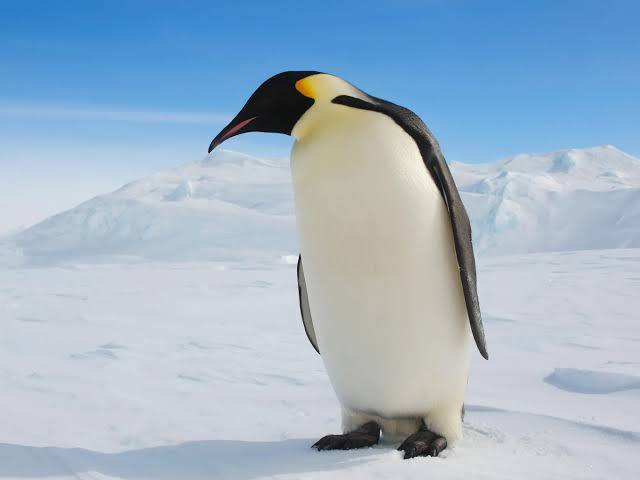
\includegraphics[width=9cm]{figures/emperor.jpeg}\\
  \caption{Caption (Figure Captions Must be Bellow the Figure).}
  \label{fig:example2}
\end{figure}

\section{Experiment}
\label{sec:results2}
~\cref{tab:example_pinguins} shows descriptive statistics of different penguins.

\begin{table}[!ht]
\centering
\caption{Caption. (Table Captions Must be Above the Tables)}
\setlength\tabcolsep{9pt}
\renewcommand{\arraystretch}{1}
\begin{tabular}{l|c|ccc}
\toprule
\textbf{Bird} & \textbf{Number of Wings} & \textbf{Location} & \textbf{Height (cm)} \\
\midrule

Emperor Penguin & \num{2}  & --- & \num{120.7} \\
King Penguin & \num{2}  & --- & \num{150.0} \\ 
Chinstrap Penguin & \num{2}  & --- & \num{50.7} \\ 
Little Blue Penguin & \num{2}  & --- & \num{30.0} \\ 

\bottomrule
\end{tabular}
\label{tab:example_pinguins}
\end{table}

\chapter{Conclusions}
\label{cha:conclusions}

This chapter summarizes the contributions of the thesis and provides an outlook into future work:

\begin{itemize}
    \item Summary
    \item Conclusions 
    \item Future work
\end{itemize}


\appendix

\chapter{Appendix}
\label{cha:appendix}

\section{Supplementary Tables}

\todo{Add supplementary tables if necessary.}

\begin{table}[!ht]
\centering
\caption{Caption. (Table Captions Must be Above the Tables)}
\setlength\tabcolsep{9pt}
\renewcommand{\arraystretch}{1}
\begin{tabular}{l|c|ccc}
\toprule
\textbf{Bird} & \textbf{Number of Wings} & \textbf{Location} & \textbf{Height (cm)} \\
\midrule

Emperor Penguin & \num{2}  & --- & \num{120.7} \\
King Penguin & \num{2}  & --- & \num{150.0} \\ 
Chinstrap Penguin & \num{2}  & --- & \num{50.7} \\ 
Little Blue Penguin & \num{2}  & --- & \num{30.0} \\ 

\bottomrule
\end{tabular}
\label{tab:example_pinguins2}
\end{table}

\clearpage
\section{Supplementary Figures}

\todo{Add supplementary figures if necessary.}

\begin{figure}[hbt!]
    \centering
     \begin{subfigure}[b]{\textwidth}
         \centering
         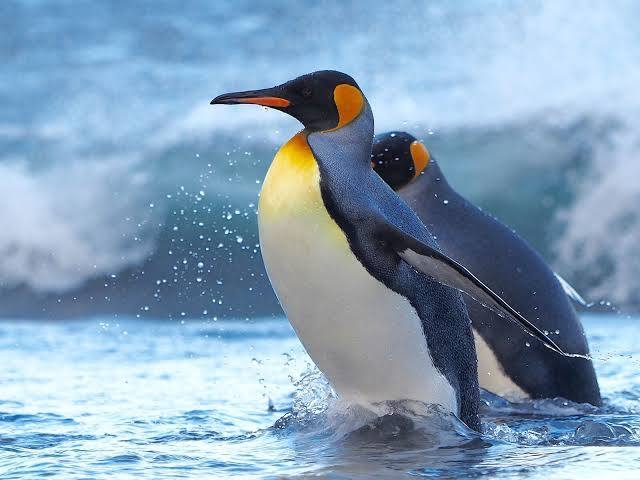
\includegraphics[width=0.5\textwidth]{figures/king.jpeg}
         \caption{King Penguin}
         \label{fig:sub1}
     \end{subfigure}
     
     \begin{subfigure}[b]{\textwidth}
         \centering
         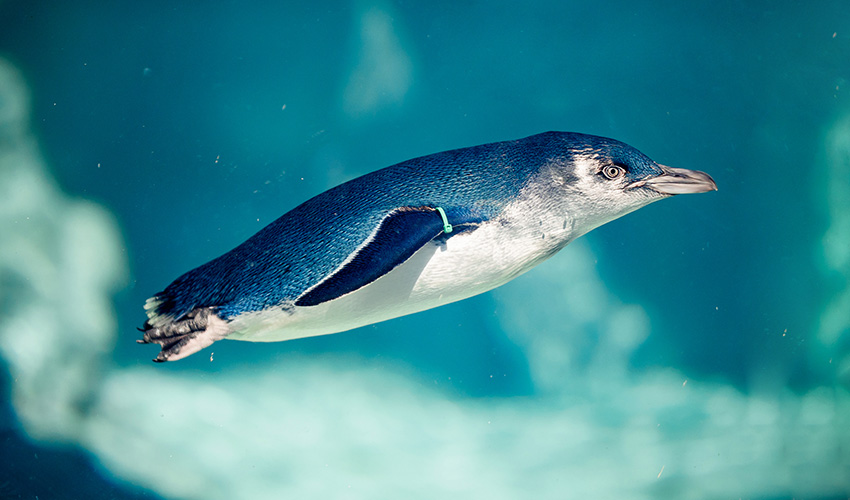
\includegraphics[width=0.5\textwidth]{figures/little_blue.jpg}
         \caption{Little Blue Penguin}
         \label{fig:sub2}
     \end{subfigure}
\caption{Penguins.}
\label{fig:example1}
\end{figure}


\backmatter

\bibliographystyle{plain}
\bibliography{refs}

\end{document}
